\section{Case study}\label{sec:caseStudy}
In this section we show the application of the proposed UML bridge to a non-trivial case study based on the SysML profile.
SysML is a general-purpose modeling language for systems engineering applications \cite{sysml}, it has been proposed by the OMG group
and supports the specification of  hardware, software, processes, and facilities of a system.
The objective of this case study is to present how each aspect of the proposed approach works in practice on SysML models.

\begin{figure}[htbp]
	\centering
		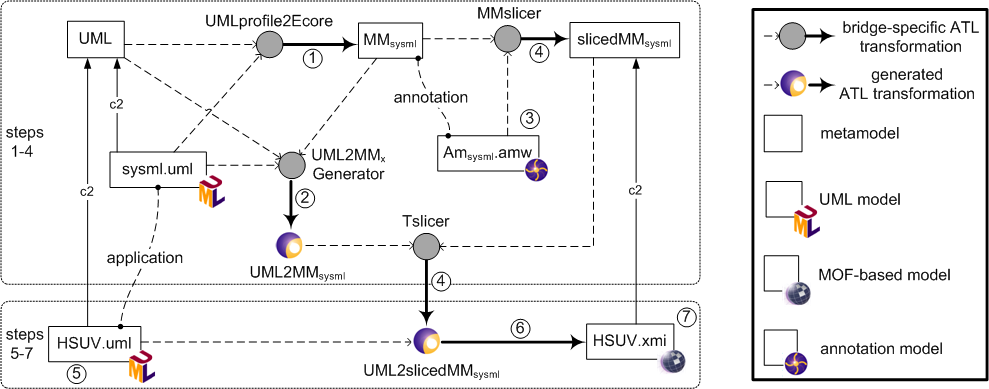
\includegraphics[width=1\textwidth]{figures/caseStudy.png}
	\caption{Overview of the HSUV case study}
	\label{fig:caseStudy}
\end{figure}

As shown in Figure \ref{fig:caseStudy}, we organized the case study as a seven-steps process:
%
\begin{enumerate}
	\item transformation of the SysML profile into a MOF metamodel called $MM_{sysml}$;
	\item automatic generation of the model transformation that creates MOF-based models from SysML-profiled models;
	\item creation of an annotation model $am_{sysml}$ to slice $MM_{sysml}$;
	\item execution of \textit{MMslicer} and \textit{Tslicer} according to the $am_{sysml}$;
	\item design of a SysML-profiled UML model ($HSUV.uml$ in figure);
	\item transformation of $HSUV.uml$ into its MOF-based counterpart ($HSUV.xmi$);
	\item development of a simple manipulation tool that works on $HSUV.xmi$.
\end{enumerate}
%
Before going into the details of each step, it is important to note that steps 1-4 are executed only once, 
then the generated ATL transformation can be re-used every time a SysML model has to be bridged.

\ivano{dire che due to space limitations non mettiamo le cose che valgono in fase di generazione, ma che qui ci focalizziamo sui modelli e la trasf finale.}

In this case study we use the Papyrus modeling tool\footnote{Papyrus UML web site: \small{\url{http://www.papyrusuml.org}}} as UML
tool. We chose it for two main reasons: (i) a SysML add-in provides support for modeling SysML-like models in Papyrus according to
the official SysML specification,
and (ii) it is based on Eclipse, so our bridge and the Papyrus tool coexist in the same modeling environment.

\textbf{Step 1.} We firstly consider the SysML profile definition made available by the Papyrus add-in,
and then we transform it into the corresponding MOF metamodel
by means of the $UMLprofile2MOF$ transformation (it is described in Section \ref{sec:metamodelLevel}). 
The resulting $MM_sysml$ metamodel is composed of XX metaclasses, YY attributes and ZZ references 
(either associations, aggregations or generalizations).

\textbf{Step 2.} In this step we execute the higher-order transformation called $UML2MM_xGenerator$ in order to obtain the
model transformation that takes as input SysML-profiled models and returns MOF-based models. The generated transformation 
($UML2MM_{sysml}$ in figure) is composed of XXX transformation rules, YYYY feature bindings, ZZZ helpers; the total size of the transformation is XXXX lines of ATL code.

\textbf{Step 3.} In order to slice the obtained metamodel and transformation, 
we (automatically) generate an annotation model by means of the second generation mechanism
(see Section \ref{sec:slicing}) by assuming that only XXX and YYY diagrams are used.
The generated annotation model ($am_{sysml}$ in figure) contains XXXX links to metaclasses like YYY, XXX, and so on.

\textbf{Step 4.} The newly created annotation model is used to execute the \textit{MMslicer} and \textit{Tslicer} transformations.
These transformations adapt $MM_{sysml}$ and $UML2MM_{sysml}$ by leaving out those elements that do not belong either to XXX or YYY diagrams. 
The adapted metamodel ($slicedMM_{sysml}$) contains XXX metaclasses, yy attributes and ZZ references. 
The size of the adapted transformation ($UML2slicedMM_{sysml}$) is XXXX lines 
of ATL code; it contains XXX transformation rules, YYYYY feature bindings and ZZZ helpers. 
The $UML2slicedMM_{sysml}$ transformation will be used to transform the initial UML model described in the next step into its 
corresponding MOF-based model.

\textbf{Step 5.} In order to XXX, we decided to reuse an already existing SysML-based UML model. So we in this case study we consider
 the example model provided in the SysML official specification and we developed it in the papyrus modeling tool.
This model represents a Hybrid gas/electric powered Sport Utility Vehicle (HSUV) by focussing on its requirements, performance, structure, and behavior. Figure \ref{fig:hsuvUML} shows a fragment of ..... \ivano{completare}. Due to space limitations, we do not provide the details of the HSUV model, however the interested reader can download and use the full UML model from our UML bridge web page. 

\begin{figure}
  \centering
  \subfloat[]{\label{fig:hsuvUML}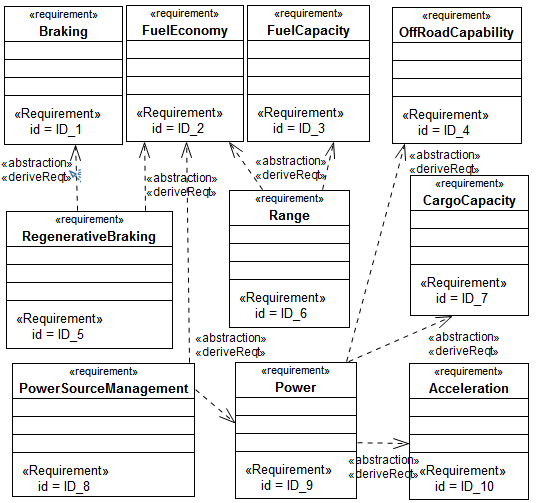
\includegraphics[scale=0.4]{figures/hsuvUML.png}}
 \hspace{10mm}
  \subfloat[]{\label{fig:hsuvMOF}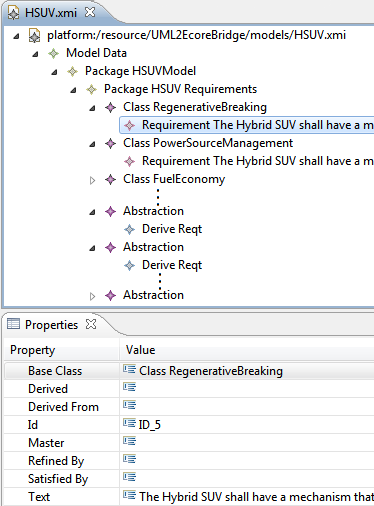
\includegraphics[scale=0.4]{figures/hsuvMOF.png}}
  \caption{HSUV system: a UML model (a) and its corresponding MOF-based model (b)}
  \label{fig:hsuv}
\end{figure}
%
\textbf{Step 6.} At this point we can execute the $UML2slicedMM_{sysml}$ Transformation in order to obtain a MOF-based representation
of the HSUV model. Figure \ref{fig:hsuvMOF} shows a fragment of the .... \ivano{completare}.

\textbf{Step 7.} In this step we provide an extremely simplified manipulation tool that operates on bridge MOF models. 
It is important to point up that technical accuracy and XXX are not in the focus of this part of the case study, 
its main goal is to show as clearly as possible how manipulation tools may benefit from our UML bridge. 
More specifically, the manipulation tool is implemented as an ATL transformation that XXXX...
%
\begin{lstlisting}[breaklines,style=AMMA,language=ATL,mathescape,rulesepcolor=\color{black},caption=ATL transformation working on MOF-based SysML models,captionpos=b,label={lst:manipulationTool}]
helper context OclAny def : UntypedGenericKernels : 
  Set(GenericKernel) = 
  MM!GenericKernel.allInstancesFrom('IN')
    ->select(x | x.type.oclIsUndefined());
...
entrypoint rule KernelTypeUpdate {
  do {
    for (e in thisModule.UntypedGenericKernels()) {
      e.type<-thisModule.createNewKernelType(e);
      thisModule.setSuperTypes(e.type);
      ...
}}}
\end{lstlisting}

Listing \ref{lst:manipulationTool} shows an excerpt of this transformation. 
\ivano{il dominio della trasf e' piccolo e ben definito, accedere agli stereotipi e' piu facile, accedere ai valori dei tagged value e' piu facile}

\ivano{il case study e' riproducibile: basta andare sulla webpage e scaricarsi i modelli e trasf descritti in questa sezione}



%The objective of this case study is to present how the UML bridge works at both metamodeling and modeling
%abstraction layers, how the slicing mechanism works in practice, and how a XXX manipulation tool may benefit from
%the application of our approach.